\chapter[Mixer Circuit using BJT]{Mixer (Frequency Converter) Circuit using BJT}
\section*{Aim}
To design and set up a frequency converter circuit to produce an output frequency ($f_0$) which is the difference frequency between the two input frequency, ($f_{1}-f_{2}$).
\section*{Theory}
A mixer or frequency mixer is a nonlinear electrical circuit that creates new frequencies from two signals applied to it. In its most common application, two signals at frequencies $f_1$ and $f_2$ are applied to a mixer, and it produces new signals at the sum $f_1 + f_2$ and difference $f_1 - f_2$ of the original frequencies. Other frequency components (like $f_1 \pm 2f_2$ may also be produced in a practical frequency mixer.\footnote{\url{http://en.wikipedia.org/wiki/Frequency_mixer}}

The most important application of mixers are in superhetrodyne receivers where the very high carrier frequency is down converted to an intermediate frequency. This is done by mixing the carrier frequency with a locally generated oscillator frequency to get an output frequency which is the difference between local oscillator frequency and incoming signal frequency, ie the intermediate frequency. In widely used AM receivers the local oscillator frequency is so chosen with respect to carrier frequency such that their difference is a constsnt intermediate frequency of 455kHz.\\
\begin{center}
$f_{IF}=f_{oscillator}-f_{carrier}=455 kHz$
\end{center}
The mixer output which contains all image frequencies of $f_1 \pm nf_2$ is filtered to obtain the required difference frequency $f_1-f_2$.
\section*{Design}
Let the input at the base be 10kHz($f_1$) signal and at the emitter be 9 kHz($f_2$) signal such that the output contains their sum and difference frequencies. The output can be low pass filtered to obtain the difference frequency $f_1-f_2=1 \ KHz$.
\\ Choose Transistor BC107. See \ref{BC107} for its datasheet details. 
\noindent Take $V_{CC}=12 V$ and $I_C=2 mA$ under dc biasing conditions.

\noindent For Class A mode of operation, let
\begin{equation}
V_{CE}=\ 50\% \ of V_{CC}=\ 6 V
\end{equation}
\begin{equation}
V_{RC}=\ 40\% \ of V_{CC}=\ 4.8 V
\end{equation}
\begin{equation}
V_{RE}=\ 10\% \ of V_{CC}=\ 1.2 V
\end{equation}

 \paragraph{Design of Emitter and Collector Resistors}
 
\begin{equation}
R_C=\ \frac{V_{RC}}{I_C}=\ \frac{4.8V}{2mA}=\ 2.4 k \Omega. \approx 2.2k\Omega (\ standard \ resistor\  value)
\end{equation}
\begin{equation}
R_E=\ \frac{V_{RE}}{I_E}=\ \frac{1.2V}{2mA}=\ 600 \Omega. \approx 560\Omega (\ standard \ resistor \ value)
\end{equation}
\noindent (Since $I_C \approx I_E =2mA$)

\paragraph{Design of Potential divider resistors $R_1$ and $R_2$ \\}
\noindent At dc bias point,
\begin{equation}
I_B=\ \frac{I_C}{h_{fEmin}}=\ \frac{2mA}{110} \approx 20 \mu A
\end{equation}

\noindent Let the current through $R_1$ be $10I_B$ and that through $R_2$ be $9I_B$ such that $I_B$ flows through the base of BC107.
\begin{equation}
I_{R1}=\ 10I_B=\ 200 \mu A
\end{equation}
\begin{equation}
I_{R2}=\ 9I_B=\ 180 \mu A
\end{equation}



\noindent Voltage across resistor $R_2$ is,
\begin{equation}
V_{R2}= V_{RE} +V_{BEactive} =\ 1.2V+0.6V=\ 1.8 V
\end{equation}
 \begin{equation}
R_2=\ \frac{V_{R2}}{I_2}= \ \frac{1.8V}{180 \mu A}=\ 100k\Omega
\end{equation}

\noindent Voltage across resistor $R_1$ is,
\begin{equation}
V_{R1}= V_{CC} +V_{R2} =\ 12V-1.8V=\ 10.2 V
\end{equation}
 \begin{equation}
R_1=\ \frac{V_{R1}}{I_1}= \ \frac{10.2V}{200 \mu A}=\ 51k\Omega \approx 47 k\Omega (\ standard \ resistor \ value)
\end{equation}

\paragraph{Design of coupling capaciors\\}
\noindent $C_1 = 1 \mu F$ and $C_E = 0.1 \mu F $

\paragraph{Design of Filter Circuit\\}

\noindent Inorder to lowpass filter the output signal choose the upper cut-off frequency be $f_o$=1.5kHz so that the required output 1 kHz appears in the pass band.
\noindent The cut-off frequency of lowpass filter is,
\begin{equation}
f_o=\ \frac{1}{2\pi R_fC_f}=1.5\ kHz
\end{equation}
\noindent where $R_f$ and $C_f$ are the passive filter components.

Choose $R_f=\ 10k\Omega$
\begin{equation}
\therefore C_f=\frac{1}{2\pi R_f f_o} \approx 0.01 \mu F.
\end{equation}
\noindent Choose $\pi$ filter configuration for better performance.
\section*{Components and Equipments required}
Function Generators(2), CRO(1), Connection wires, Breadboard, Probes.
\\BC107 (1)
\\ $47k\Omega,\  10k\Omega\ (2),\ 560\Omega,\,\ 2.2k\Omega ,\ 10k\Omega (2) $- Resistors
\\ $ 1\mu F (1),\ 0.1\mu F (1), \ 0.01\mu F (3)$ - Capacitor
\section*{Circuit Diagram}
See Figure \ref{mixer} for circuit diagram.
\begin{figure}[h]
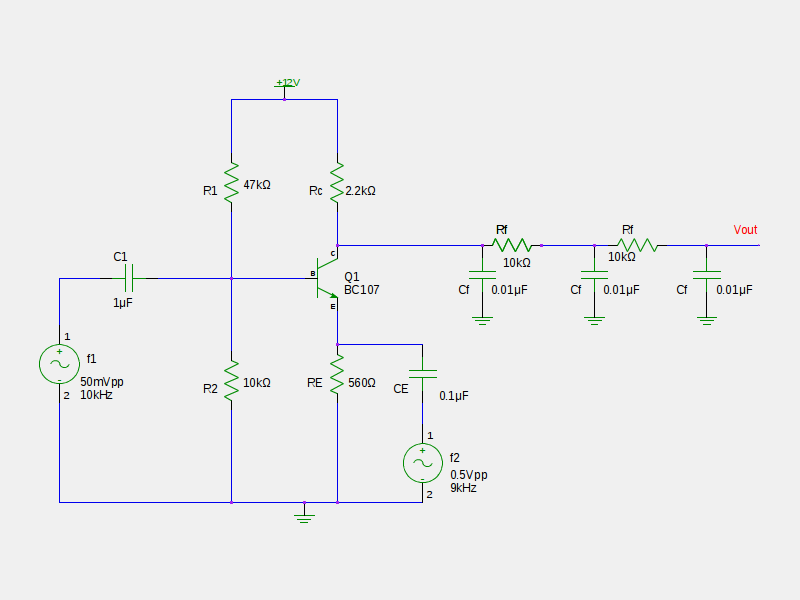
\includegraphics[width=\textwidth, height=10cm, trim=3cm 3cm 3cm 3cm,clip=true]{mixer.png}
\caption{Circuit Diagram for Mixer circuit using BJT}
\label{mixer}
\end{figure}
\section*{Procedure}
\begin{enumerate}
\item
Make connections as per the circuit diagram.
\item
Feed $f_1$ and $f_2$ with amplitudes as shown in the circuit diagram and frequencies 10 kHz and 9 kHz respectively.
\item
Observe the filtered output frequency on a CRO.
\item
Repeat with frequencies changed to 20 kHz and 19kHz  (50 kHz and 49 kHz)and observe it in CRO. Verify that the circuit gives the difference frequency of 1 kHz at the output.
\item
Plot the input and output signals on a graph sheet. 

\end{enumerate}
\section*{Observation}
From the graph find the frequency of the output signal.\\
\textcolor{red}{Model graph to be added}
\section*{Result}
The mixer circuit using BJT was set up and output was verified from signals observed on a CRO.


